\documentclass{article}\usepackage[]{graphicx}\usepackage[]{color}
% maxwidth is the original width if it is less than linewidth
% otherwise use linewidth (to make sure the graphics do not exceed the margin)
\makeatletter
\def\maxwidth{ %
  \ifdim\Gin@nat@width>\linewidth
    \linewidth
  \else
    \Gin@nat@width
  \fi
}
\makeatother

\definecolor{fgcolor}{rgb}{0.345, 0.345, 0.345}
\newcommand{\hlnum}[1]{\textcolor[rgb]{0.686,0.059,0.569}{#1}}%
\newcommand{\hlstr}[1]{\textcolor[rgb]{0.192,0.494,0.8}{#1}}%
\newcommand{\hlcom}[1]{\textcolor[rgb]{0.678,0.584,0.686}{\textit{#1}}}%
\newcommand{\hlopt}[1]{\textcolor[rgb]{0,0,0}{#1}}%
\newcommand{\hlstd}[1]{\textcolor[rgb]{0.345,0.345,0.345}{#1}}%
\newcommand{\hlkwa}[1]{\textcolor[rgb]{0.161,0.373,0.58}{\textbf{#1}}}%
\newcommand{\hlkwb}[1]{\textcolor[rgb]{0.69,0.353,0.396}{#1}}%
\newcommand{\hlkwc}[1]{\textcolor[rgb]{0.333,0.667,0.333}{#1}}%
\newcommand{\hlkwd}[1]{\textcolor[rgb]{0.737,0.353,0.396}{\textbf{#1}}}%
\let\hlipl\hlkwb

\usepackage{framed}
\makeatletter
\newenvironment{kframe}{%
 \def\at@end@of@kframe{}%
 \ifinner\ifhmode%
  \def\at@end@of@kframe{\end{minipage}}%
  \begin{minipage}{\columnwidth}%
 \fi\fi%
 \def\FrameCommand##1{\hskip\@totalleftmargin \hskip-\fboxsep
 \colorbox{shadecolor}{##1}\hskip-\fboxsep
     % There is no \\@totalrightmargin, so:
     \hskip-\linewidth \hskip-\@totalleftmargin \hskip\columnwidth}%
 \MakeFramed {\advance\hsize-\width
   \@totalleftmargin\z@ \linewidth\hsize
   \@setminipage}}%
 {\par\unskip\endMakeFramed%
 \at@end@of@kframe}
\makeatother

\definecolor{shadecolor}{rgb}{.97, .97, .97}
\definecolor{messagecolor}{rgb}{0, 0, 0}
\definecolor{warningcolor}{rgb}{1, 0, 1}
\definecolor{errorcolor}{rgb}{1, 0, 0}
\newenvironment{knitrout}{}{} % an empty environment to be redefined in TeX

\usepackage{alltt}

\usepackage[OT4]{polski}
\usepackage[utf8]{inputenc}
\usepackage[T1]{fontenc}
\usepackage[top=2.5cm, bottom=2.5cm, left=2cm, right=2cm]{geometry}
\usepackage{graphicx}
\usepackage{float}
\usepackage[colorlinks=true, linkcolor=blue]{hyperref}
\usepackage{amsmath}
\usepackage{amssymb}



\title{Lista 1}
\author{Mikołaj Langner, Marcin Kostrzewa}
\date{31.3.2021}
\IfFileExists{upquote.sty}{\usepackage{upquote}}{}
\begin{document}

\maketitle

\section{Wstęp}
W niniejszym sprawozdaniu zajmować się będziemy analizą \ldots

\section{Etap I}
Wczytajmy dane z pliku i przeprowadźmy ich wstępną analizę i obróbkę:

\begin{knitrout}
\definecolor{shadecolor}{rgb}{0.969, 0.969, 0.969}\color{fgcolor}\begin{kframe}
\begin{alltt}
\hlstd{df} \hlkwb{<-} \hlkwd{read.csv}\hlstd{(}\hlstr{'churn.txt'}\hlstd{,} \hlkwc{stringsAsFactors} \hlstd{=} \hlnum{TRUE}\hlstd{)}
\hlstd{df}\hlopt{$}\hlstd{Area.Code} \hlkwb{=} \hlkwd{as.factor}\hlstd{(df}\hlopt{$}\hlstd{Area.Code)}
\end{alltt}
\end{kframe}
\end{knitrout}

\begin{itemize}

\item poznajmy rozmiar naszych danych:
\begin{knitrout}
\definecolor{shadecolor}{rgb}{0.969, 0.969, 0.969}\color{fgcolor}\begin{kframe}
\begin{alltt}
\hlkwd{dim}\hlstd{(df)}
\end{alltt}
\begin{verbatim}
## [1] 3333   21
\end{verbatim}
\end{kframe}
\end{knitrout}
--- są więc 21 zmienne i 3333 obserwacji;

\item sprawdźmy ich typ:
% latex table generated in R 4.0.4 by xtable 1.8-4 package
% Sun Mar 28 22:27:56 2021
\begin{table}[H]
\centering
\begin{tabular}{rl}
  \hline
 & Typ zmiennej \\ 
  \hline
State & factor \\ 
  Account.Length & integer \\ 
  Area.Code & factor \\ 
  Phone & factor \\ 
  Int.l.Plan & factor \\ 
  VMail.Plan & factor \\ 
  VMail.Message & integer \\ 
  Day.Mins & numeric \\ 
  Day.Calls & integer \\ 
  Day.Charge & numeric \\ 
  Eve.Mins & numeric \\ 
  Eve.Calls & integer \\ 
  Eve.Charge & numeric \\ 
  Night.Mins & numeric \\ 
  Night.Calls & integer \\ 
  Night.Charge & numeric \\ 
  Intl.Mins & numeric \\ 
  Intl.Calls & integer \\ 
  Intl.Charge & numeric \\ 
  CustServ.Calls & integer \\ 
  Churn. & factor \\ 
   \hline
\end{tabular}
\caption{Hello} 
\label{tab:tabela1}
\end{table}


\item sprawdźmy czy pojawiają się wartości brakujące:
\begin{knitrout}
\definecolor{shadecolor}{rgb}{0.969, 0.969, 0.969}\color{fgcolor}\begin{kframe}
\begin{alltt}
\hlkwd{sum}\hlstd{(}\hlkwd{sapply}\hlstd{(df,} \hlkwa{function}\hlstd{(}\hlkwc{x}\hlstd{)} \hlkwd{sum}\hlstd{(}\hlkwd{is.na}\hlstd{(x))))}
\end{alltt}
\begin{verbatim}
## [1] 0
\end{verbatim}
\end{kframe}
\end{knitrout}

\item usuńmy dane pełniące rolę indentyfikatora:
\begin{knitrout}
\definecolor{shadecolor}{rgb}{0.969, 0.969, 0.969}\color{fgcolor}\begin{kframe}
\begin{alltt}
\hlstd{df} \hlkwb{<-} \hlkwd{subset}\hlstd{(df,} \hlkwc{select}\hlstd{=}\hlopt{-}\hlstd{Phone)}
\end{alltt}
\end{kframe}
\end{knitrout}

\end{itemize}

Teraz podzielimy zmmienne ze względu na typ oraz wykonamy kilka wykresów, które pomogą w zauważeniu pewnych zależności.
\begin{knitrout}
\definecolor{shadecolor}{rgb}{0.969, 0.969, 0.969}\color{fgcolor}\begin{kframe}
\begin{alltt}
\hlkwd{library}\hlstd{(ggplot2)}
\hlkwd{library}\hlstd{(GGally)}
\hlkwd{library}\hlstd{(tidyr)}
\hlkwd{library}\hlstd{(dplyr)}
\hlkwd{library}\hlstd{(EnvStats)}
\hlkwd{library}\hlstd{(DescTools)}
\end{alltt}
\end{kframe}
\end{knitrout}

\begin{knitrout}
\definecolor{shadecolor}{rgb}{0.969, 0.969, 0.969}\color{fgcolor}\begin{kframe}
\begin{alltt}
\hlstd{factors} \hlkwb{<-} \hlkwd{subset}\hlstd{(df,} \hlkwc{select}\hlstd{=}\hlkwd{sapply}\hlstd{(df, is.factor))}
\hlstd{numerics} \hlkwb{<-} \hlkwd{subset}\hlstd{(df,} \hlkwc{select}\hlstd{=}\hlkwd{sapply}\hlstd{(df,} \hlkwa{function}\hlstd{(}\hlkwc{x}\hlstd{)} \hlopt{!}\hlkwd{is.factor}\hlstd{(x)))}
\end{alltt}
\end{kframe}
\end{knitrout}

\begin{knitrout}
\definecolor{shadecolor}{rgb}{0.969, 0.969, 0.969}\color{fgcolor}\begin{kframe}
\begin{alltt}
\hlstd{numerics} \hlkwb{<-} \hlkwd{data.frame}\hlstd{(numerics,} \hlkwc{Churn.} \hlstd{= df}\hlopt{$}\hlstd{Churn.)}
\end{alltt}
\end{kframe}
\end{knitrout}

\begin{knitrout}
\definecolor{shadecolor}{rgb}{0.969, 0.969, 0.969}\color{fgcolor}\begin{kframe}
\begin{alltt}
\hlstd{continuous} \hlkwb{<-} \hlkwd{subset}\hlstd{(numerics,} \hlkwc{select}\hlstd{=}\hlkwd{sapply}\hlstd{(numerics,} \hlkwa{function}\hlstd{(}\hlkwc{x}\hlstd{)} \hlopt{!}\hlkwd{is.integer}\hlstd{(x)))}
\hlkwd{ggpairs}\hlstd{(continuous,}
        \hlkwc{lower}\hlstd{=}\hlkwd{list}\hlstd{(}\hlkwc{continuous}\hlstd{=}\hlkwd{wrap}\hlstd{(}\hlstr{"points"}\hlstd{,} \hlkwc{alpha}\hlstd{=}\hlnum{.4}\hlstd{,} \hlkwc{size}\hlstd{=}\hlnum{.01}\hlstd{)))}
\end{alltt}
\end{kframe}

{\centering 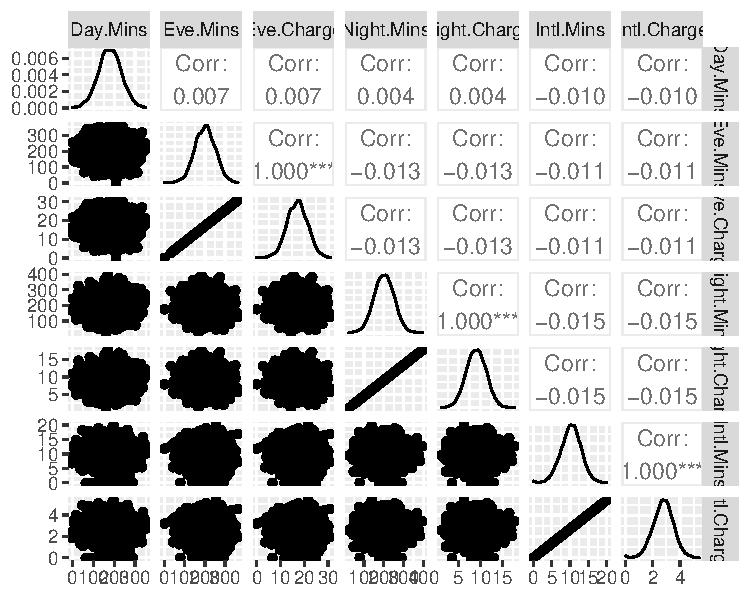
\includegraphics[width=\maxwidth]{figure/Pair_plot_for_continuous_variables-1} 

}



\end{knitrout}

\begin{knitrout}
\definecolor{shadecolor}{rgb}{0.969, 0.969, 0.969}\color{fgcolor}\begin{kframe}
\begin{alltt}
\hlkwd{ggplot}\hlstd{(}\hlkwd{gather}\hlstd{(factors,} \hlstr{"key"}\hlstd{,} \hlstr{"value"}\hlstd{,} \hlopt{-}\hlstd{Churn.),} \hlkwd{aes}\hlstd{(value,} \hlkwc{color}\hlstd{=Churn.))} \hlopt{+}
  \hlkwd{geom_bar}\hlstd{(}\hlkwc{position}\hlstd{=}\hlstr{'dodge'}\hlstd{,} \hlkwd{aes}\hlstd{(}\hlkwc{y}\hlstd{=(..count..)}\hlopt{/}\hlkwd{sum}\hlstd{(..count..)))} \hlopt{+}
  \hlkwd{facet_wrap}\hlstd{(}\hlopt{~}\hlstd{key,} \hlkwc{scales}\hlstd{=}\hlstr{'free'}\hlstd{)}
\end{alltt}
\end{kframe}

{\centering 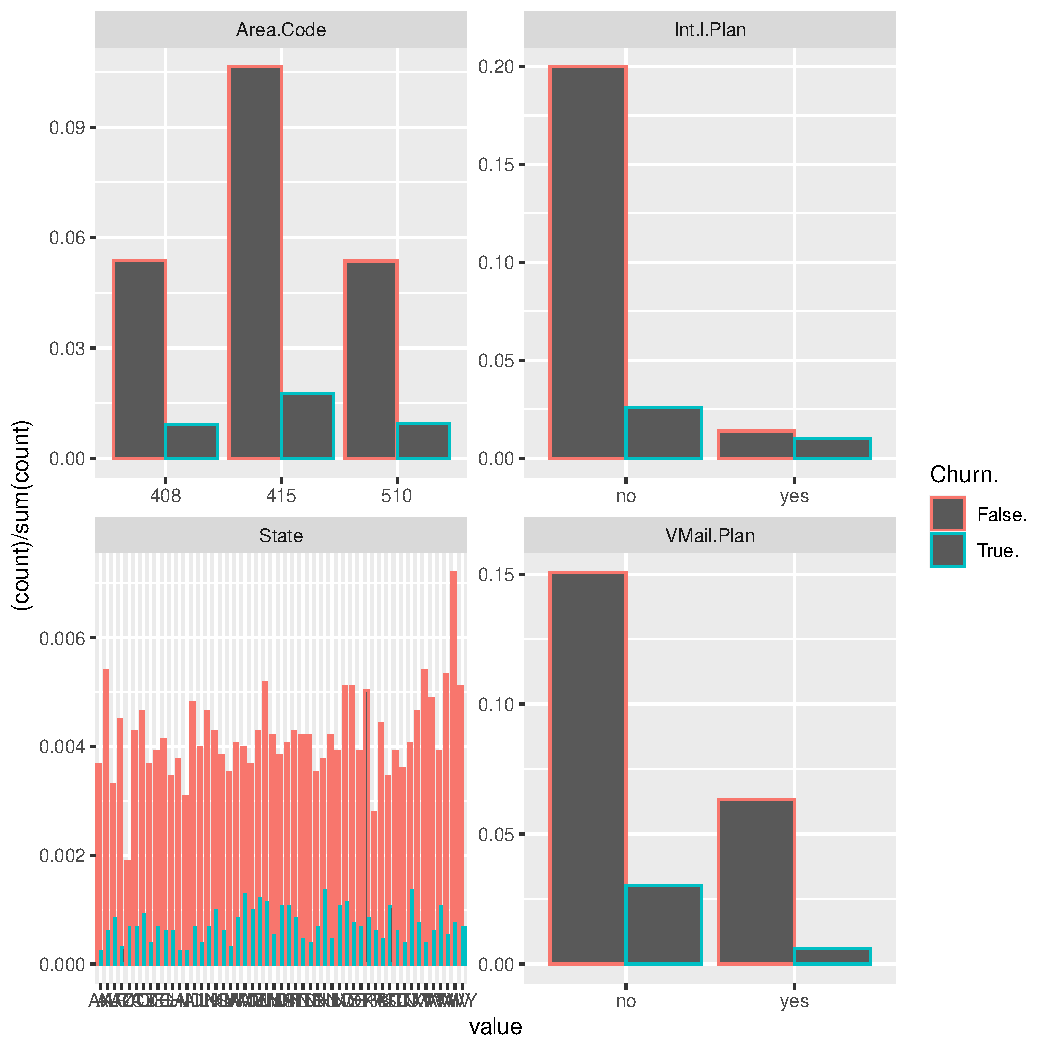
\includegraphics[width=\maxwidth]{figure/Overviews_plots_grouped-1} 

}


\begin{kframe}\begin{alltt}
\hlkwd{ggplot}\hlstd{(}\hlkwd{gather}\hlstd{(numerics,} \hlstr{"key"}\hlstd{,} \hlstr{"value"}\hlstd{,} \hlopt{-}\hlstd{Churn.),} \hlkwd{aes}\hlstd{(value,} \hlkwc{color}\hlstd{=Churn.))} \hlopt{+}
  \hlkwd{geom_freqpoly}\hlstd{(}\hlkwd{aes}\hlstd{(}\hlkwc{y}\hlstd{=..density..))} \hlopt{+}
  \hlkwd{facet_wrap}\hlstd{(}\hlopt{~}\hlstd{key,} \hlkwc{scales}\hlstd{=}\hlstr{'free'}\hlstd{)}
\end{alltt}
\end{kframe}

{\centering 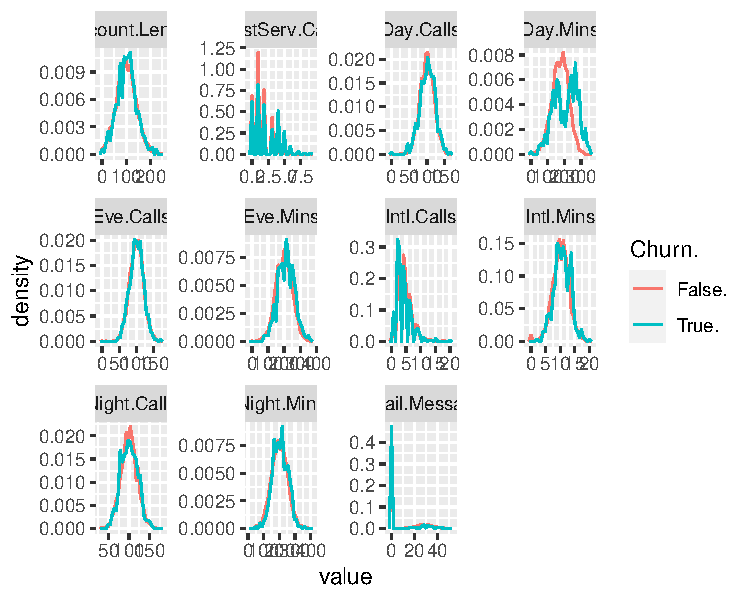
\includegraphics[width=\maxwidth]{figure/Overviews_plots_grouped-2} 

}


\begin{kframe}\begin{alltt}
\hlkwd{ggplot}\hlstd{(}\hlkwd{gather}\hlstd{(numerics,} \hlstr{"key"}\hlstd{,} \hlstr{"value"}\hlstd{,} \hlopt{-}\hlstd{Churn.),} \hlkwd{aes}\hlstd{(value,} \hlkwc{color}\hlstd{=Churn.))} \hlopt{+}
  \hlkwd{geom_boxplot}\hlstd{(}\hlkwd{aes}\hlstd{(}\hlkwc{x}\hlstd{=value))} \hlopt{+}
  \hlkwd{facet_wrap}\hlstd{(}\hlopt{~}\hlstd{key,} \hlkwc{scales}\hlstd{=}\hlstr{'free'}\hlstd{)}
\end{alltt}
\end{kframe}

{\centering 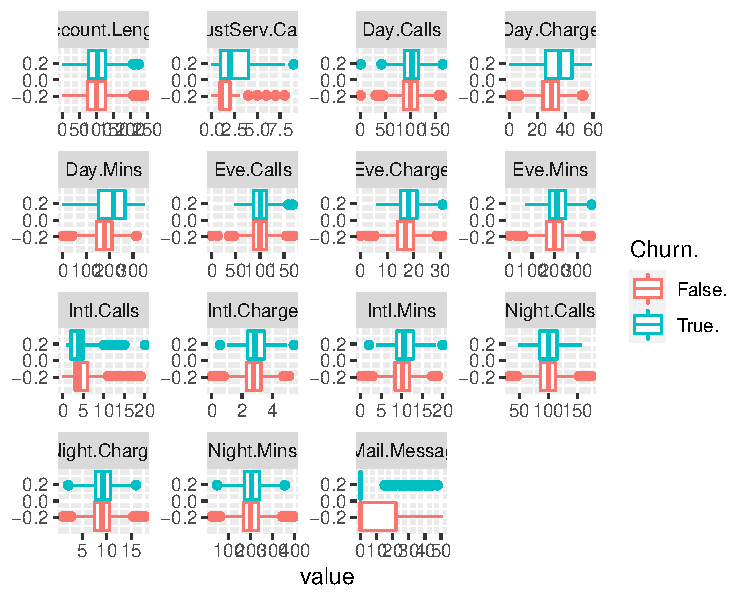
\includegraphics[width=\maxwidth]{figure/Overviews_plots_grouped-3} 

}



\end{knitrout}

Po przeanalizowaniu wykresów, decydujemy się na dalszą analizę następujących zmiennych:
\begin{itemize}
  \item ilościowych:
    \begin{itemize}
    \item CustServ.Calls,
    \item Day.Mins,
    \item Eve.Mins;
    \end{itemize}
  \item jakościowych
    \begin{itemize}
    \item Int.l.Plan,
    \item VMail.Plan,
    \item Churn.
    \end{itemize}
\end{itemize}

\section{Etap II}


\section{Etap III}


\section{Etap IV}


\end{document}
